\documentclass[border=5pt]{standalone}
\usepackage[T1]{fontenc}
\usepackage{tikz}

\definecolor{horseshoe}{HTML}{65780B}
\definecolor{atlantic}{HTML}{466A9F}
\definecolor{garnet}{HTML}{73000A}
\definecolor{rose}{HTML}{CC2E40}
\definecolor{warmgrey}{HTML}{676156}
\definecolor{bk70}{HTML}{5C5C5C}
\definecolor{bk30}{HTML}{C7C7C7}

\begin{document}
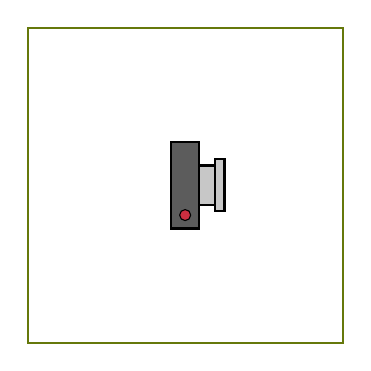
\begin{tikzpicture}
  \useasboundingbox (-2,-2) rectangle (2,2);
  \draw[horseshoe, thick] (-2,-2) rectangle (2,2);

  % Camera scope — centered at origin, pointing right
  \begin{scope}[shift={(0,0)}, scale=1]
    % Body (taller, narrower)
    \fill[bk70] (-0.18,-0.55) rectangle (0.18,0.55);
    \draw[black, thick] (-0.18,-0.55) rectangle (0.18,0.55);

    % Lens barrel (narrower rectangle extending right)
    \fill[bk30] (0.18,-0.25) rectangle (0.38,0.25);
    \draw[black, thick] (0.18,-0.25) rectangle (0.38,0.25);

    % Lens flare (wider rectangle at the tip)
    \fill[bk30] (0.38,-0.33) rectangle (0.5,0.33);
    \draw[black, thick] (0.38,-0.33) rectangle (0.5,0.33);

    % Shutter button (red circle on top)
    \fill[rose] (0.0,-0.38) circle (0.07);
    \draw[black, thin] (0.0,-0.38) circle (0.07);
  \end{scope}

\end{tikzpicture}
\end{document}
